\documentclass[a4paper]{article}


\usepackage[T1]{fontenc}    
\usepackage[utf8]{inputenc} 
\usepackage{textcomp}      
\date{} 					
\author{}                   
\usepackage{geometry}		
\geometry{ left=2cm, right=2cm, top=2cm, bottom=4cm, bindingoffset=5mm}

\usepackage{graphicx}
\usepackage{xcolor}
\usepackage{hyperref} 
\usepackage{fancyhdr}												
\pagestyle{fancy}
\fancyhf{}
\fancyhead[R]{2973140 - Felix Bühler  \\ 2893121 - Jan Leusmann \\  3141241 - Jamie Ullerich}
\fancyhead[L]{Scientific Visualisation \\ Sommersemester 2019 }
\renewcommand{\headrulewidth}{0.5pt} 				

\title{Exercise 4}

\begin{document}
	
	\maketitle 
	\thispagestyle{fancy}
	

	
	\section*{Exercise 4.1 - Grid Types}
	
	\section*{Exercise 4.2 - Voronoi Diagram}
	
	The computation of a voronoi cell can be compared to the nearest neighbour interpolation. 
	The function value of the cell can be assigned to all point inside it. 
	These points are closer to every sample inside the cell than to all other points. \\ \linebreak
	The geometrical dual of a voronoi diagram is the delaunay graph. 
	If two voronoi cells share an edge, two nodes of the delaunay graph are connected. 
	One of these two nodes must be in the first and the corresponding one in the second voronoi cell. 
	This relationship is shown in Figure \ref{fig:diagram}. 
	For example, the nodes $x_{3}$ and $x_{2}$ are connected because the corresponding voronoi cells are next to each other and therefore share and edge. 
	
	\begin{figure}[h!]
		\centering
		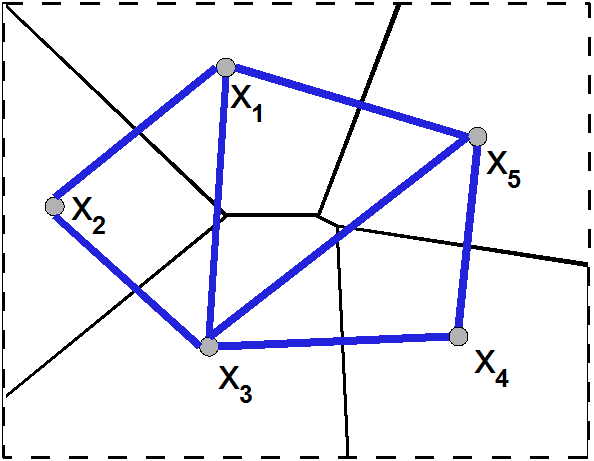
\includegraphics[width=0.3\linewidth]{diagram}
		\caption{Picture from lecture vis04 slide 15.}
		\label{fig:diagram}
	\end{figure}
	
	\section*{Exercise 4.3 - Bi-linear Interpolation}
	
	$f_{j} = \frac{7 - 3}{7 - 2} \cdot 0.4 + \frac{3 - 2}{7 - 2} \cdot 0.1 = 0.8 \cdot 0.4 + 0.2 \cdot 0.1 = 0.34$ \\ \linebreak
	$f_{j + 1}  = 0.8 \cdot 0.2 + 0.2 \cdot (-0.2) = 0.12$ \\ \linebreak
	$f = \frac{5 - 3.5}{5 - 3} \cdot 0.34 + \frac{3.5 - 3}{5 - 3} \cdot 0.12 = 0.255 + 0.03 = \textbf{0.285}$
	
	\section*{Exercise 4.4 - ParaView: Color Mapping}
	
	
	
\end{document}